\documentclass{article}
\usepackage{graphicx} % Required for inserting images
\usepackage[T1]{fontenc}
\usepackage[utf8]{inputenc}
\usepackage[polish]{babel}
\usepackage{lmodern}
\usepackage[hidelinks]{hyperref} 
\usepackage{booktabs}
\usepackage{csvsimple}
\usepackage[table]{xcolor}
\usepackage{array}
\usepackage{colortbl}
\usepackage{amsmath}
\usepackage{geometry}
\usepackage{pdfpages}
\usepackage{enumitem}
\usepackage{ragged2e}
\usepackage{float}
\usepackage{adjustbox}
\usepackage{float}
\usepackage{placeins}

\begin{document}

\begin{titlepage}
\newgeometry{left=1.6in, right=2in}
\vspace*{1.5cm}

\noindent  \textcolor{gray}{\large Piotr Marszałek, Julia Łaszyca, Aleksandra Skibińska} \\
\vspace{1cm}

\noindent \textbf{\Large Część laboratoryjna Biofizyki - Ćwiczenie 2} \\
\vspace{0.5cm}

\noindent {\large Określanie potencjału dyfuzji\textbf{} } \\


Listopad 2026 \\

\vspace{0.4cm}
\noindent Politechnika Gdańska \\
Wydział Elektroniki, Telekomunikacji i Informatyki \\
Katedra Inżynierii Biomedycznej \\

\begin{figure}[b]
    
\includegraphics[width=0.44\textwidth]{logol.jpg}
\end{figure}
\end{titlepage}




\section*{Aparatura użyta do wykonania zadania}
    \begin{itemize}
        \item Komputer osobisty z programem symulacyjnym równania Nernsta
    \end{itemize}
    
\section*{Sprawozdanie właściwe}

\section{Cele doświadczenia}
    \begin{itemize}
        \item Zapoznanie się ze zjawiskami transportu ładunków elektrycznych w ciele
        \item Pomiar potencjału dyfuzyjnego
        \item Określenie i porównanie przepuszczalności błony dla kationów sodu ($Na^{+})$
        \item Nakreślenie zależności potencjału dyfuzyjnego od temperatury wybranej różnicy stężeń
    \end{itemize}

    
\section{Krótki punktowy opis przebiegu ćwiczenia}
    \begin{enumerate}[label=(\alph*)]
        \item Wyznaczono wartość potencjału dyfuzyjnego dla danych eksperymentalnych wraz z niepewnościami.\newline
        \item Obliczono wartość teoretyczną potencjału dyfuzji dla każdego pomiaru. \newline
        \item Wykonano symulację dla tych samych stężeń Na. (W przypadku stężeń w pomiarze 4 i 5 odpowiednio przeskalować stężenie tak, żeby symulacja była możliwa)\newline
        \item Porównano potencjał dyfuzyjny wyznaczony eksperymentalnie, zasymulowany oraz wyliczony teoretycznie.  \newline
        \item Wyznaczono za pomocą symulatora dla dowolnie wybranej różnicy stężeń zależność potencjału dyfuzyjnego od temperatury. (Narysować wykres i dopasować go odpowiednią funkcją)\newline
    \end{enumerate}

\section{Dane oraz wzory}
    \begin{table}[!h]
        \centering
        \csvautotabular[
            separator=semicolon,
            respect underscore=true
            ]{cw2tab1.csv}
        \caption{Dane ćwiczeniowe}
        \label{tab:tab1}
    \end{table}
    
    \begin{table}[!h]
        \centering
        \csvautotabular[
            separator=semicolon,
            respect underscore=true
            ]{cw2tab2.csv}
        \caption{Przedłużenie tabeli \ref{tab:tab1}}
        \label{tab:tab2}
    \end{table}
    
\FloatBarrier
    \begin{equation}
        \Delta\varphi=-\frac{RT}{F}\left[\frac{t_+}{z_+}-\frac{t_-}{z_-}\right]ln\frac{c_2}{c_1}
        \label{eq:henderson}
    \end{equation}


    \begin{center}
        Równanie Hendersona \\
    \end{center}
    $\Delta\varphi$: potencjał dyfuzyjny\\
    $t_{+/-}$: liczby przenoszenia dla kationu/anionu\\
    $c_{1/2}$: stężenia elektrolitów po różnych stronach membrany\\
    $R, T, F$: stała gazowa, temperatura absolutna[$^\circ K$], stała Faradaya\\
        
    
\section{Pomiary: 1, 2, oraz 3}

    \subsection{Wyznaczyć wartość potencjału dyfuzyjnego dla danych eksperymentalnych wraz z niepewnościami.}

    \subsection{Obliczyć wartość teoretyczną potencjału dyfuzji dla każdego pomiaru. }

    \subsection{Pomiary z symulatora}


        \begin{table}[!h]
            \centering
            \begin{tabular}{|c|c|c|}\hline
                 lp.&proporcja $[\frac{kom.1}{kom.2}]$ &pomiar 3 \\[3pt] \hline
                 1&  $\frac{10}{1}$& $58.8[mV]$ \\ [3pt]\hline
                 2&  $\frac{100}{1}$& $117.5[mV]$ \\ [3pt]\hline
                 3&  $\frac{100}{10}$& $58.8[mV]$ \\ [3pt]\hline
                 4&  $\frac{600}{6}$& $117.5[mV]$ \\ [3pt]\hline
                 5&  $\frac{600}{60}$& $58.8[mV]$ \\ [3pt]\hline
            \end{tabular}
            \caption{Pomiary z symulatora}
            \label{tab:symulator}
        \end{table}
        \FloatBarrier
        Wyniki potencjałów z tabeli \ref{tab:symulator} pokazują, że symulator prawdopodobnie zaokrągla wyniki\\[1\baselineskip]
        W idealnym środowisku symulatora margines błędu wynosi zero, więc dla równych proporcji otrzymujemy równe pomiary.

        
        
\section{Zależność potencjału dyfuzyjnego od temperatury dla różnicy stężeń $\frac{kom.1}{kom.2}=\frac{27}{10}$}
    \begin{figure}[!h]
        \centering
        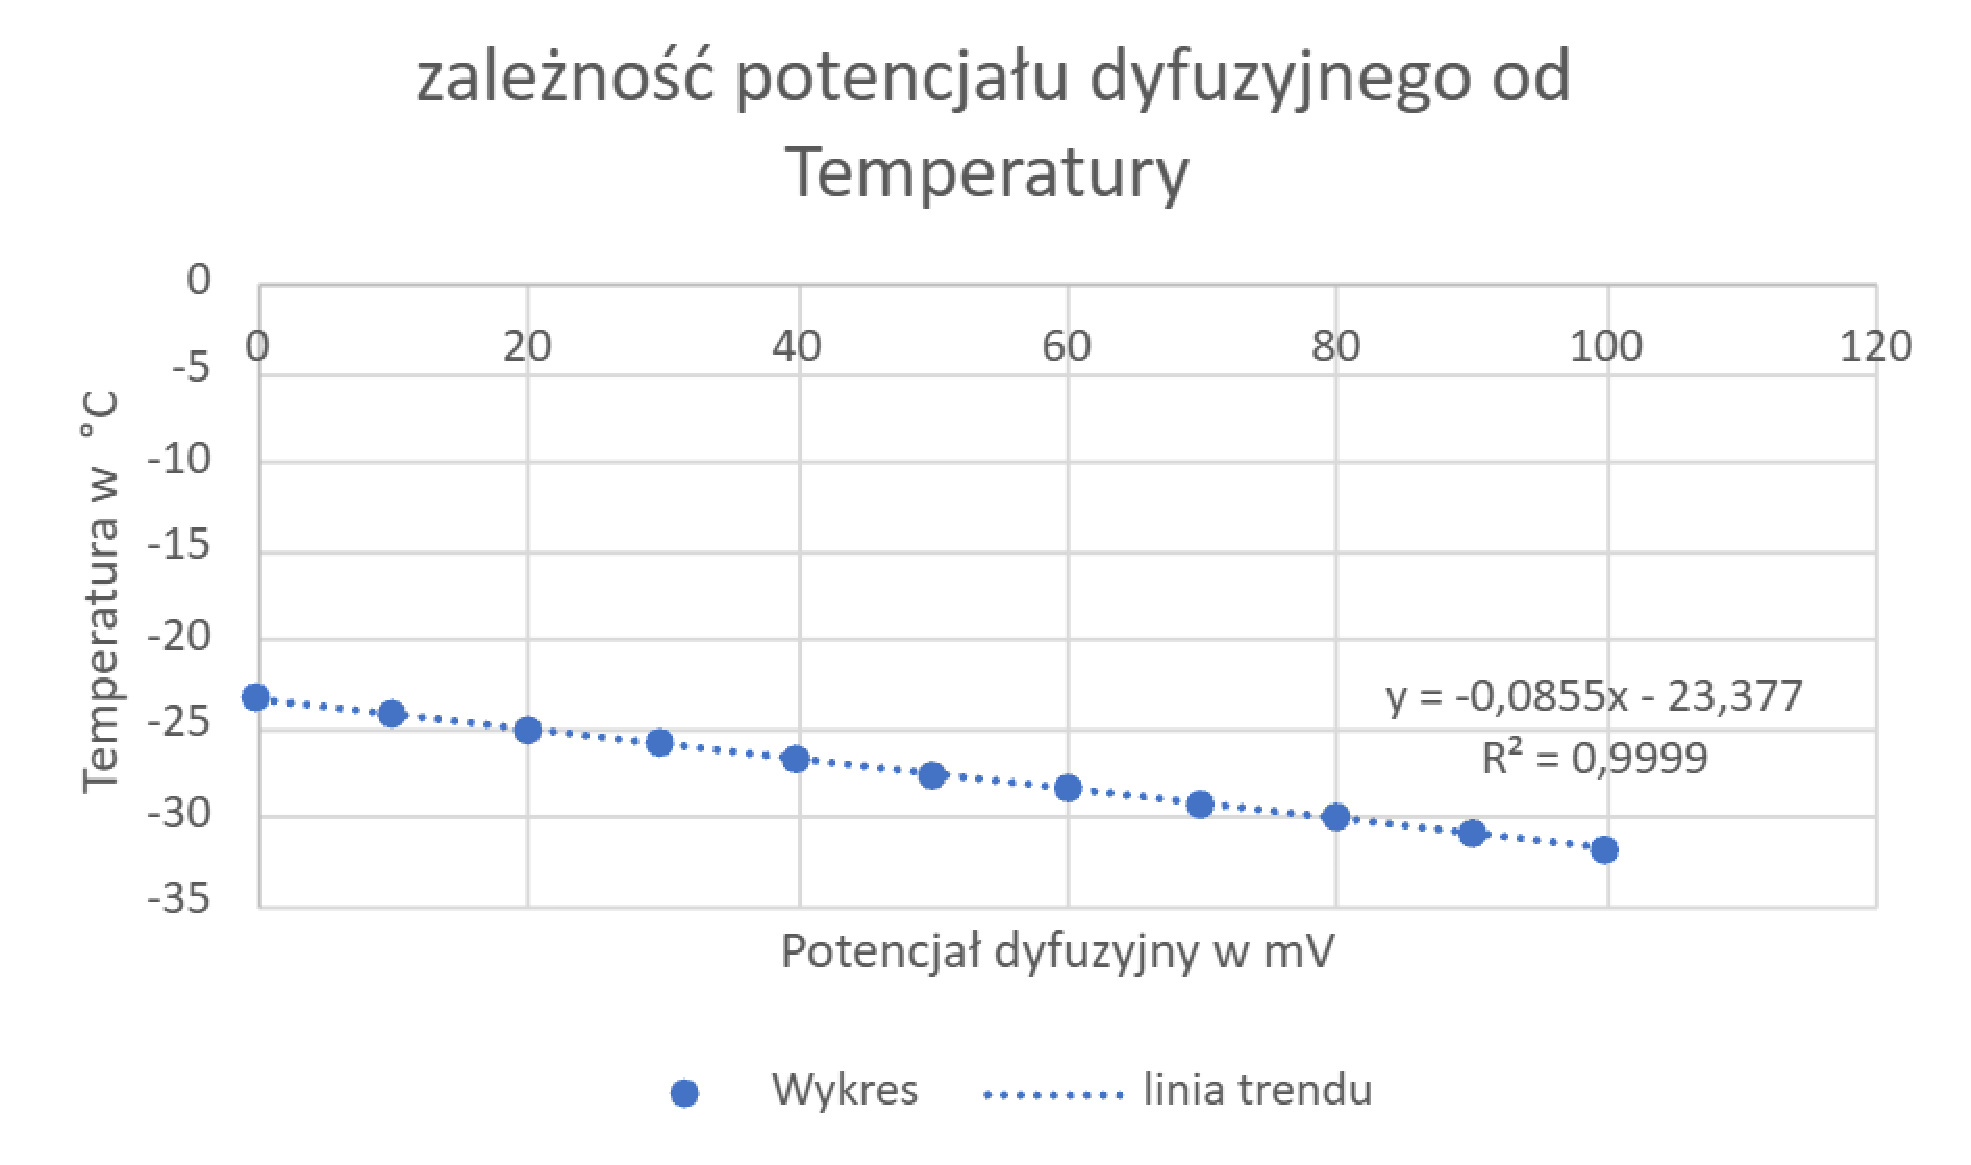
\includegraphics[width=0.9\linewidth]{screenshots.pdf}
        \caption{Wykres zależności potencjału dyfuzyjnego od temperatury dla zadanej różnicy stężeń}
        \label{fig:wykres}
    \end{figure}
    \FloatBarrier

    Jak widać na rysunku \ref{fig:wykres}, zgodnie ze wzorem \ref{eq:henderson}, wartość potencjału dyfuzyjnego maleje wraz ze zwiększaniem się wartości temperatury.\\[1\baselineskip]
    Przy zmienności temperatury potencjał spada liniowo ze względu na ujemny współczynnik kierunkowy.\\[1\baselineskip]
    Warto zauważyć, że wyidealizowane pomiary otrzymane z symulatora wyprodukowały niemal idealną prostą, której parametr $R^2 \approx 1$

\section*{Wnioski z pracy}
    \begin{itemize}
        \item tutaj  
        \item dajcie
        \item wnioski
    \end{itemize}

    Praca została wykonana bez pomocy sztucznej inteligencji
\end{document}
 
